\documentclass[11pt,letterpaper]{article}

\usepackage{palatino}
\usepackage{graphicx}
\usepackage{wrapfig}

\begin{document}

\author{Burke Libbey}
\title{COMP 3370 Assignment 1}

\maketitle

\section{Design Documentation}

\subsection{Architechture Description}

The CPU consists of several registers and two distinct memory spaces, for separate storage of program code and data. All registers and memory locations are 16 bits in size, modeled using \texttt{word\_t}, which is typedef'd to \texttt{uint16\_t}.

All the registers and memory spaces are contained in a single \texttt{struct cpu} or \texttt{cpu\_t}. I probably should have made it a global variable, but instead, a pointer to this struct is passed around quite a bit.

\hspace{20mm}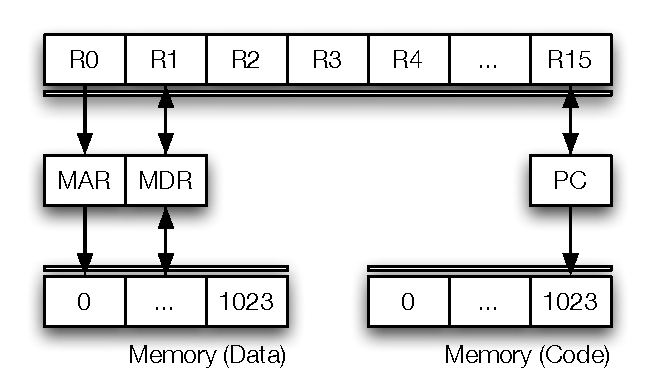
\includegraphics[width=80mm]{datapath.pdf}
 
Like the spec suggests, I have \texttt{R0..R15} and \texttt{PC}. I've also added \texttt{MAR} and \texttt{MDR} to interface with memory as per a suggestion in class.

\newpage

\subsection{Execution}

\begin{wrapfigure}{r}{60mm}
  \begin{center}
   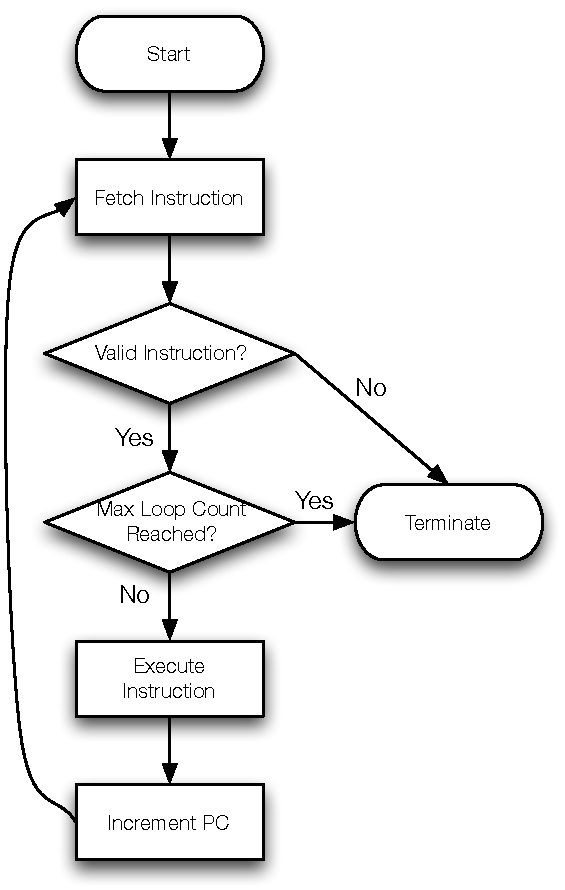
\includegraphics[width=60mm]{flow.pdf}
  \end{center}
\end{wrapfigure}

After initializing the CPU, the main loop will continue to fetch instructions, parse out the opcode and operands, execute instructions, and increment the program counter. It will terminate when an invalid instruction is reached, or an infinite loop is encountered.

Each time an instruction is fetched, both operands are extracted, whether or not they are of any use, and a function is then called to modify the CPU's state using the opcode and operands.

\subsection{Program Implementation}

The main program file is \texttt{src/sim.c}. This contains the main loop and various functions related to reading and parsing input to initialize the simulator.

\texttt{src/architecture.\{c,h\}} contains a description of the CPU architecture. The \texttt{cpu\_t} struct contains all of the registers and memory locations available to a program for this CPU. The makeCpu() function initializes a \texttt{cpu\_t} with sane default values (mostly zeroes, \texttt{0xFFFF} for code space).

\texttt{src/bitmacros.h} contains convenience macros for extracting data from interestingly-sized types. \texttt{OPCODE}, for example, extracts the 6 bits representing the opcode from an instruction value (16 bits).

Finally \texttt{src/instructions.\{c,h\}} defines operations for each instruction supported by the CPU. Instructions are stored as an array of function pointers. Each invocation of \texttt{INSTRUCTION} defines a function. These are later loaded into an array by \texttt{makeInstructionTable()} to return to the main program.

\newpage

\section{Test Programs}
\subsection{Test 1}
This program calculates Fibonacci numbers. It stores $0$ in \texttt{Data[0]} and $1$ in \texttt{Data[1]}, then $Fib(n)$ in \texttt{Data[n]}, up to $Fib(30)$.

\subsection{Test 2}
This program searches a set of data for a value. It will search up to \texttt{Data[1]} words for the value in \texttt{Data[0]}. Once it is found the index at which it was found is stored in \texttt{Data[0]}. If no match is found, $0$ is stored instead. It's worth noting, I guess, that if the target is in the first value searched, $0$ is returned as the result, so it looks like an error.

\subsection{Test 3}
This program loops infinitely, since the \texttt{JR} jumps back to one instruction \textit{after} the \texttt{BEQ} it was probably ``supposed'' to jump to.

\subsection{Test 4}
This program... doesn't even pretend to make sense? I guess it would terminate if \texttt{Data[1]} was $0$... instead it just loops, adding to \texttt{R5} then comparing \texttt{R4}.

\subsection{Test 5}
This is a very similar search to the one in question 2, except it will never terminate if the data is not found.

\subsection{Test 6}
This program multiplies the numbers in \texttt{Data[0]} and \texttt{Data[1]}, storing the result to \texttt{Data[0]}. Obviously, overflow is a concern.

\subsection{Test 7}
This program essentially multiplies $9$ and $-1$, storing the result in \texttt{Data[0]} and \texttt{Data[1]}. It uses a mostly-out-of-spec register-to-register move operation.


\end{document}